\chapter{Introduction}

\section{Background}

With a history spanning well over a half century, hypersonic flight continues to be a topic of significant research interest\ \cite{parker.control.2007,gibson.adaptive.2009,kothari.reusable.2010,dalle.envelope.2011,brocanelli.unstartrecovery.2012}.
Air-breathing hypersonic vehicles are particularly attractive due to their potential to serve as high speed passenger transports and long range weapon delivery systems, and provide cost-effective access to space.
Hypersonic vehicles are likely to be inherently unstable\ \cite{mcruer.hypersonic.1991,mirmirani.airbreathing.2005,bolender.hypersonicmodel.2007} and the integration of the airframe and engine in an air-breathing hypersonic vehicle contributes to additional modeling and control challenges.
With limited wind tunnel data, harsh and uncertain operating environments, poorly known physical models, and largely varying operating conditions, it is of great importance to ensure that any control scheme will be significantly robust to ensure safe operation during flight.

Unlike the transition from subsonic to supersonic flow, the physics of hypersonic flow do not differ from that of supersonic flow.
Instead, the distinction of hypersonic flow is made to stress the importance of certain physical phenomena which exist in all supersonic flows that become dominant at hypersonic speeds, typically defined to be flow at a Mach number of 5 or greater\ \cite{anderson.aerodynamics.2010}.
It wasn't until 1946, well into the study of such flow regimes, that this term was finally coined\ \cite{Tsien2012443}.
The high flight Mach numbers experienced by a hypersonic vehicle result in significant aerodynamic heating.
This aerodynamic heating can have a great impact on the material properties of the vehicle.
In addition to this coupling of aerodynamic and structural effects, the engines of air-breathing hypersonic vehicles are tightly integrated into the airframe of the vehicle, where long fore and aft sections of the vehicle make up large portions of the engine inlet and nozzle, respectively.
This tightly couples the engine dynamics with the airframe and structural dynamics as well as the aerodynamics\ \cite{chavez.flightdynamics.1994}.
The physics of hypersonic flow and these resulting interactions between all the components of the vehicle make the control of hypersonic vehicles very challenging.

A major challenge associated with the control of hypersonic vehicles, in addition to the interactions between airframe, engine, and structural dynamics, is the limited ability to accurately determine the aerodynamics characteristics\ \cite{maughmer.prediction.1989,schmidt.dynamics.1991,chavez.analytical.1994,coleman.hypersonic.2009}.
With the presence of such tight coupling between all aspects of a hypersonic vehicle, the ability to collect wind tunnel and flight data to study these interactions would be highly useful.
However, these tests are very difficult to do, and so much of the knowledge about a hypersonic vehicle's aerodynamics must come from physics-based models.
This makes accurate determination of the aerodynamic characteristics very difficult, making the design of a controller more difficult as well.

Another control challenge associated specifically with air breathing hypersonic vehicles is that of engine unstart.
Unstart is a phenomenon caused by several factors including thermal choking and insufficient air recovery at the inlet.
This ultimately leads to the upstream propagation of the shock train out of the inlet, effectively preventing air from entering the engine due to a standing normal shock in front of the isolator entrance\ \cite{curran.scramjet.2000}.
This causes an abrupt change in the pitching moment, an increase in drag, decrease in lift, loss of thrust, and potentially changes in vehicle yawing and rolling moments as well\ \cite{bolender.unstart.2009}.
If the flight path is such that it requires the GHV to unstart, the control law must be such that it can accommodate these large and sudden changes, thus ensuring stable flight can be maintained through unstart.

With all of the complex interactions between the different aircraft components, and high level of uncertainty in the models, the control of a hypersonic vehicle is very challenging.
These challenges have led to many advances in the design of flight control.

\section{History}

The science of aerodynamics was first invented in the early 1900s by Ludwig Prandtl in Germany.
The field of aerodynamics matured considerably over the next half-century, and during World War II, the Germans were beginning to approach hypersonic speeds in laboratory wind  tunnel tests at Mach 4.4, and with weapons such as the V-2 rocket approaching similar speeds\ \cite{heppenheimer.heatbarrier.2009}.
The hypersonic technology of the United States was substantially behind that of the Germans at the time, until the war ended and Wernher von Braun and his team of rocket scientists came to the United States.
Just over eleven years after the end of World War II, history was made when the X-2 became the fastest airplane ever, reaching a speed of almost Mach 3.2.
Moments after the record was broken, the plane lost control and began tumbling downwards toward Earth, destroying the plane and killing the pilot due to a mechanism known as inertial coupling\ \cite{nelson.flightcontrol.1998}.
This disaster made the consequences of not maintaining stability during high speed flight very real.

The study of hypersonics in the 1950s was also being propelled by the United States' interest in intercontinental ballistic missiles, which began with the X-17 rocket.
The accurate guidance of such missiles over long ranges was of particular importance, but it was the challenges associated with significant aerodynamic heating upon atmospheric re-entry that dominated research in this area during this time.
The first test of the X-17 took place in 1956 to investigate the re-entry of a hemispherical nose-cone, and reached a speed of Mach 12.4.
This research provided valuable information used in the Mercury program, which succeeded in putting the first American in space in 1961.
The inherently stable design of the Mercury capsule allowed safe atmospheric re-entry even without an effective control system.
While guidance, navigation and control (GNC) challenges of later hypersonic re-entry vehicles were more difficult, the effective control of atmospheric hypersonic vehicles such as the X-2 was a major problem that needed to be solved.

Following the testing of the X-2, the X-planes program continued in the late 1950s, with much of the knowledge gained through research to be used in the development of high performance fighter aircraft of the time.
One of the most notable hypersonic airplanes to ever fly, the X-15 pictured in Figure~\ref{fig:x15flying}, made its first flight in 1959.
The designers of the X-15 overcame many of the challenges associated with hypersonic flight.
The X-15 had to be very heat resistant to withstand the temperatures encountered during flight at nearly Mach 7, and the engine needed the power to propel the plane to these high speeds.
The flight envelope of the X-15 was so broad that reaction controls were used in addition to the aerodynamic control surfaces, which lost effectiveness above 100,000 feet altitude.
Transitioning between these two control systems was difficult as well.
In addition to these challenges, and more, the only significant source of aerodynamic data used in the development of the X-15 came from a single small hypersonic wind tunnel, making modeling for control especially challenging.
Despite these challenges, three variants of the X-15 made a combined total of nearly 200 flights over the next ten years following its first flight.
The third variant of the X-15, was the only of the three craft to include an adaptive controller as part of its stability augmentation system.
This adaptive controller attempted to adjust feedback gains to provide optimum angular rates as commanded by the pilot, and also provided a means to transition from aerodynamic to reaction controls, allowing the command of both control systems from a single control stick in the cockpit.
While the X-15 allowed hours of valuable flight data to be obtained, engineers were once again reminded of the consequences of faulty designs when the MH-96 adaptive controller aboard the X-15 failed to reduce the feedback gains upon re-entry, setting up a violent pitch oscillation which destroyed the aircraft and killed the pilot.

 \begin{figure}[h]
  \begin{center}
    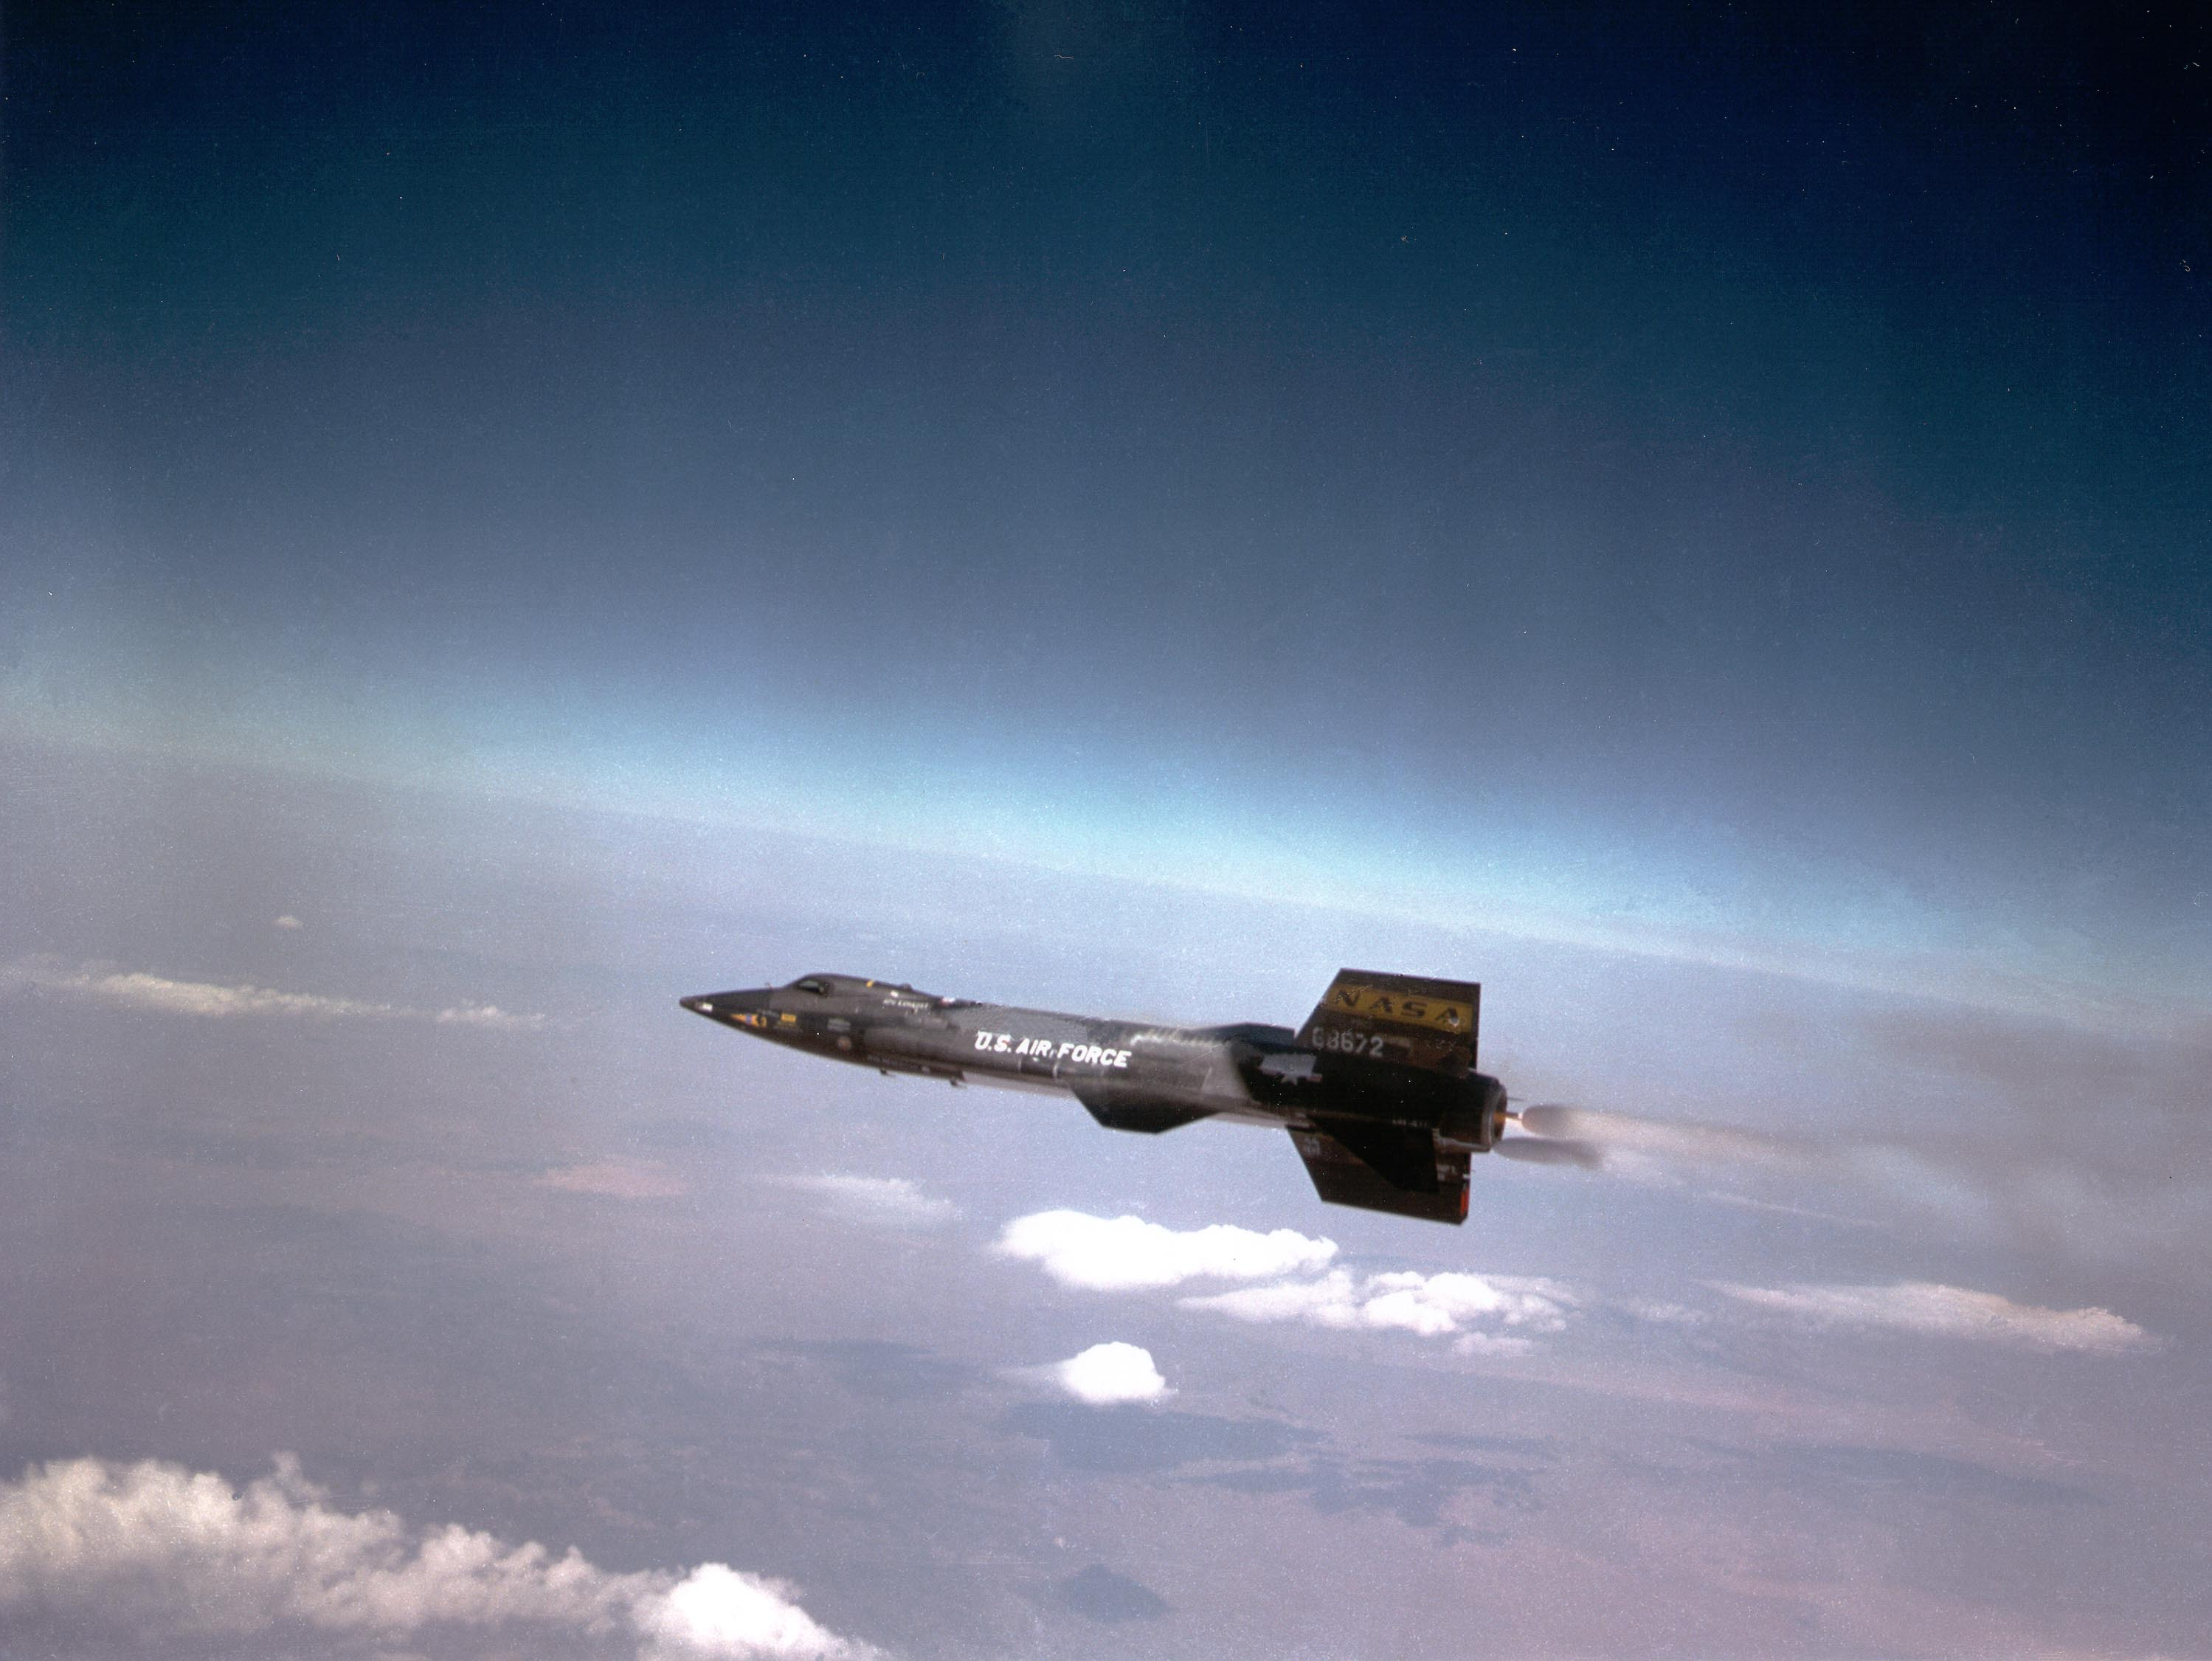
\includegraphics[width=3.5in]{\figurepath/x15flying.jpg}
    \caption{North American X-15\label{fig:x15flying}}
  \end{center}
\end{figure}

Toward the end of the X-15's career, there was a building interest in a new, advanced air-breathing propulsion system for hypersonic flight, as opposed to the rocket propulsion used on the X-15 and its predecessors.
This Hypersonic Research Engine (HRE) was to utilize concepts first disclosed by The Johns Hopkins Universities' Applied Physics Lab in 1959, as part of a project known as Supersonic Combustion Ramjet Missle (SCRAM).
The scramjet engines were initialy designed as pods, much like conventional turbofans on commercial and transport aircraft.
Early plans called for a podded scramjet to be fitted on the X-15, but it was quickly realized that this would not be possible.
To make scramjets practical for use in flight, the engine would have to be integrated intimately in the airframe, using the fore and aft sections of the vehicle as part of the inlet and nozzle of the scramjet.
Development of scramjet technology was pushed forward in the early 1980s in part by the U.S. Air Force, in order to develop a single-stage-to-orbit vehicle to deliver military weapons systems to space.
This ultimately led to the National Aero-Space Plane (NASP) program, and the design of the 160 foot long Rockwell X-30.
This program lasted over ten years and lead to many advances in scramjet propulsion research and the study of flexible hypersonic vehicles, but no X-30 were ever built.

\begin{figure}[h]
  \begin{center}
    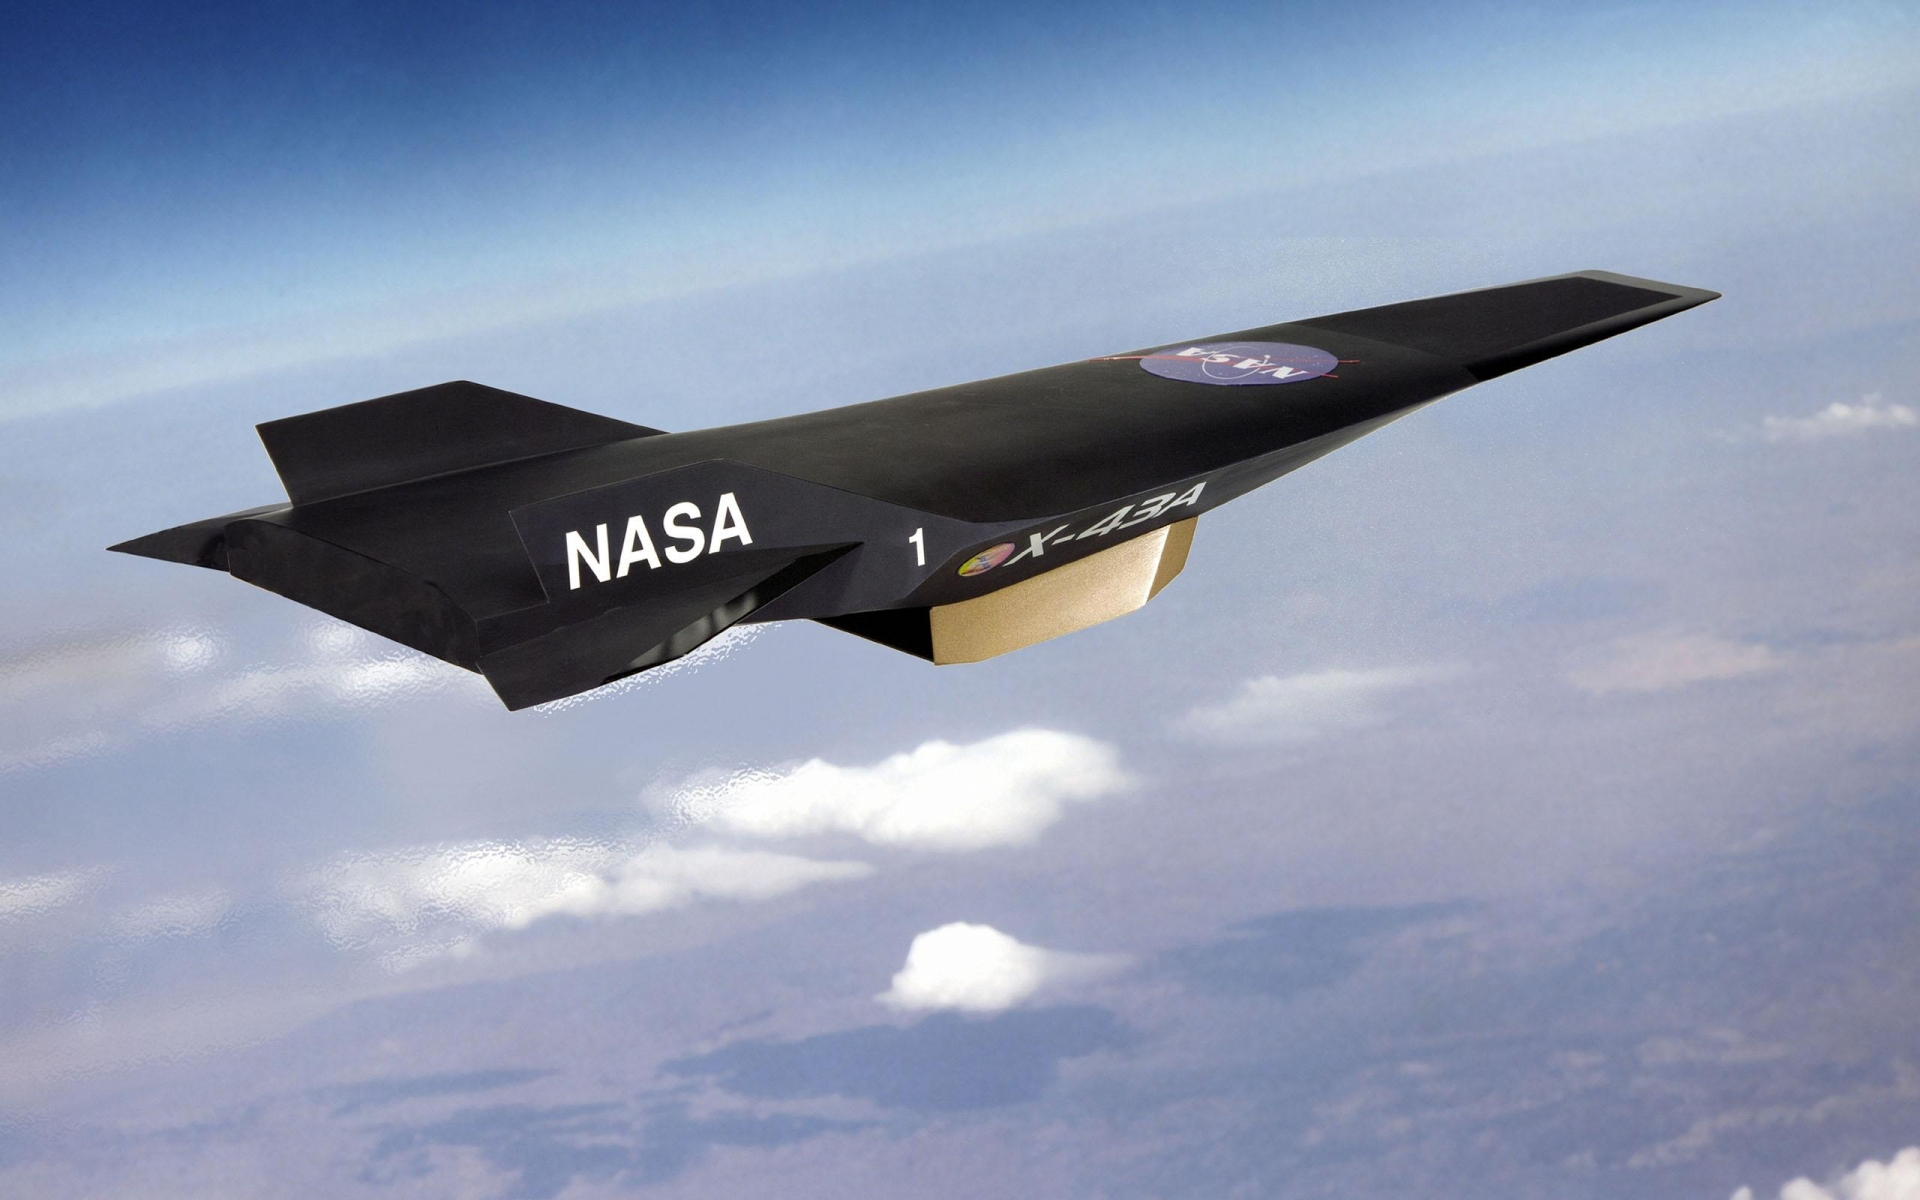
\includegraphics[width=3.5in]{\figurepath/nasa_x43.jpg}
    \caption{NASA X-43A}
  \end{center}
\end{figure}

Hypersonic research slowed for some years, until scramjet research emerged again in the early 1990s as part of a collaboration between the United States and Russia.
This collaboration saw scramjets mounted aboard rockets being tested in flight.
Control again became a critical challenge in hypersonic flight, this time in the control of the engines.
Fuel delivery had to be controlled precisely to keep the engines operating in supersonic combustion mode, and avoid a condition known as unstart.
Control systems aboard these rocket-mounted scramjets were designed to monitor pressures within the engines and adjust fuel flow to prevent unstart, but the early control systems were not yet ready for this demanding challenges.
An all-American effort at practical scramjet powered hypersonic flight was born in 1996 under the name Hyper-X\ \cite{freeman.hyperx.1997}.
Hyper-X was an eight year NASA program with the goal of demonstrating the viability of air-breathing hypersonic flight.
The demonstrator vehicle for this program, the X-43, was 12 feet long, and 5 feet wide.
The first flight took place in June 2001 and failed, but in March 2004 the X-43A became the first vehicle to ever be propelled during hypersonic flight by an air-breathing engine, reaching a speed of Mach 6.8 for 11 seconds.
The third flight in November 2004 lasted 10 seconds and reached a speed of Mach 9.6.
These ground breaking flights demonstrated the practicability of a scramjet powered hypersonic vehicle, and are alongside the X-15 in terms of importance in the history of hypersonic flight.

In the 1990s and 2000s, many hypersonics programs have been introduced, including HyTECH, HyShot, HyCause, HIFiRE, and more.
The most notable platform since the X-43A was the X-51, built by Boeing and managed by the U.S. Air Force Research Lab (AFRL).
While the X-43A demonstrated the feasibility of scramjet powered flight, a new record was set by the X-51 in 2010 by maintaining scramjet powered flight at 5 for 140 seconds.
The second X-51 flight took place in 2011 and ended early due to unstart, and during the third test flight the X-51 lost control and fell into the ocean.
History was made once again in May 2013, when the X-51 made the longest air-breathing hypersonic flight, maintaining Mach 5.1 for 240 seconds under its own power.

\begin{figure}[h]
  \begin{center}
    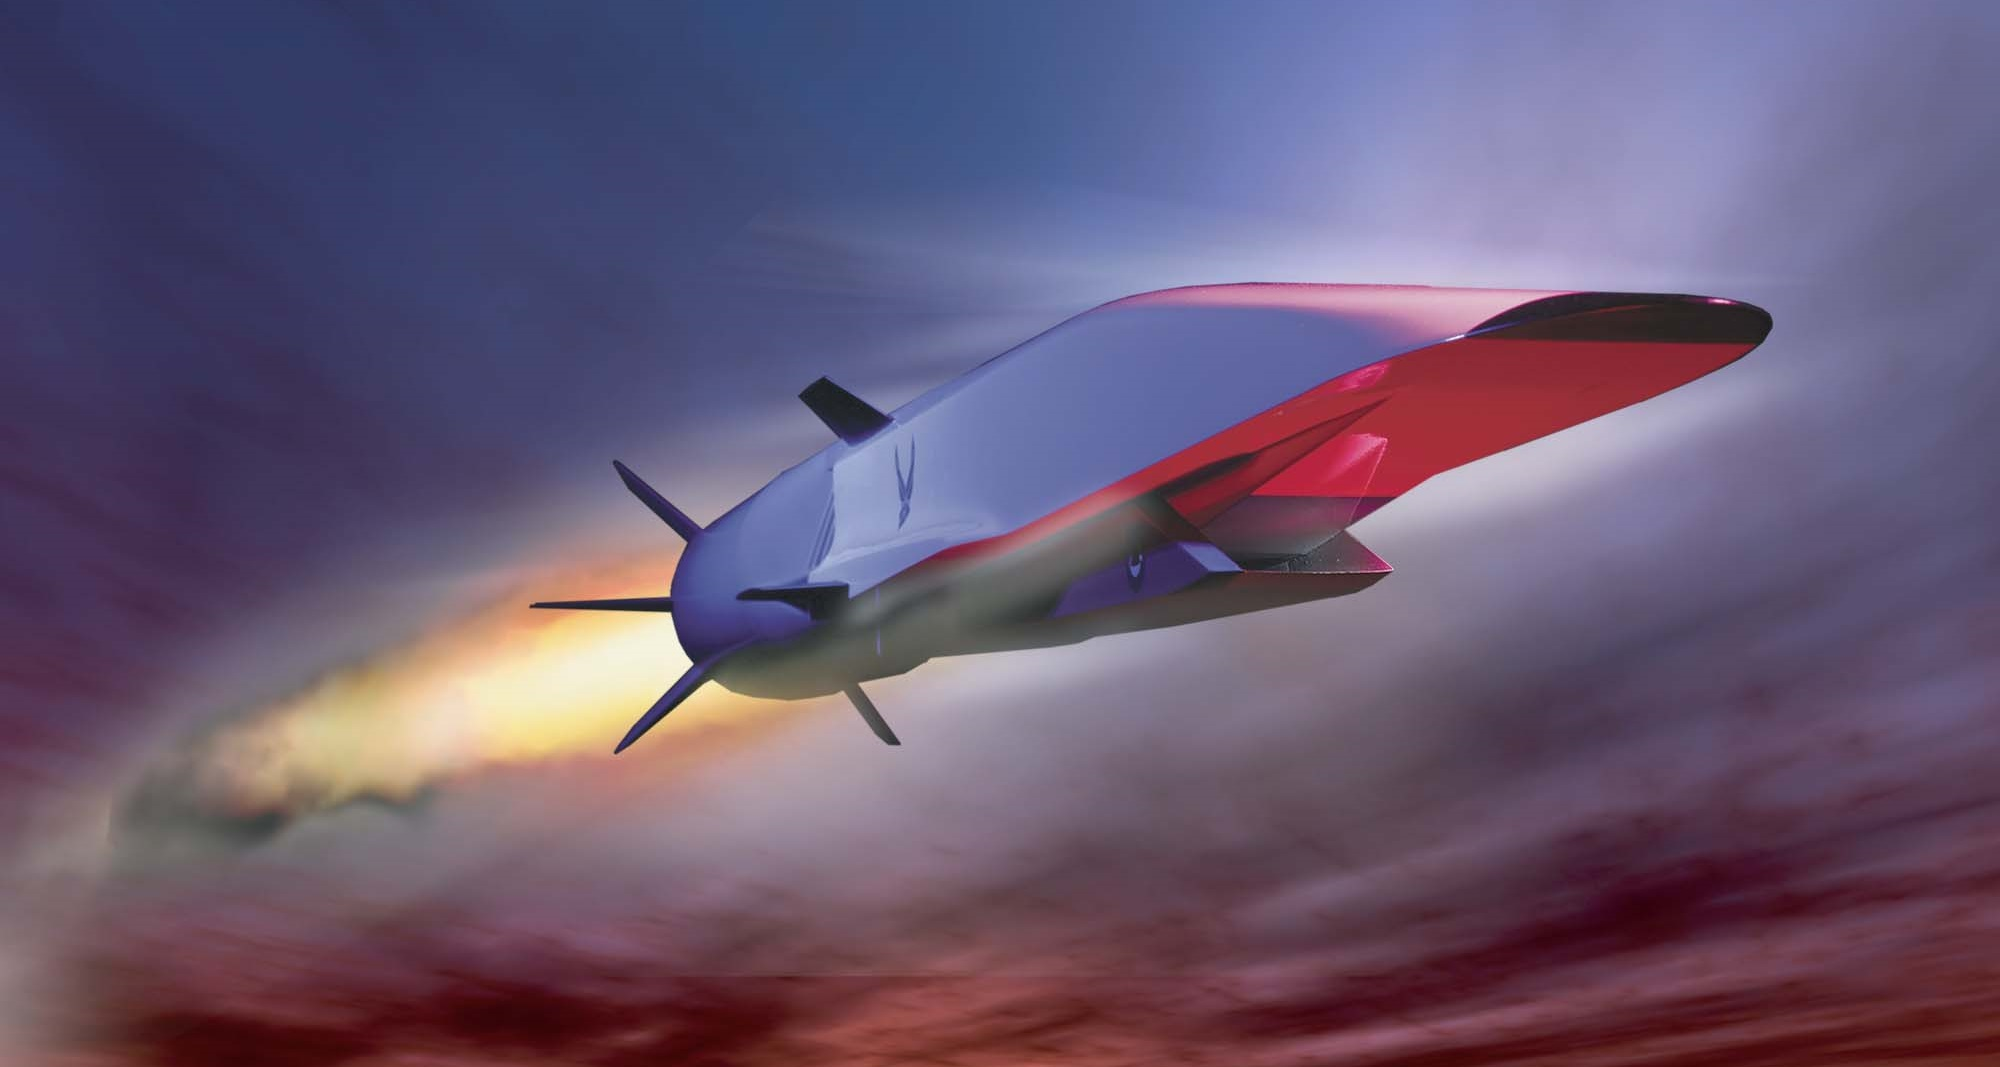
\includegraphics[width=3.5in]{\figurepath/boeing_x51_v3.jpg}
    \caption{Boeing X-51 waverider}
  \end{center}
\end{figure}

The history of hypersonic flight is still in the making, with current research centered around the sustained flight of air-breathing vehicles.
The previous trajectories flown by aircraft such as the X-15, X-43 and X-51 were fairly benign in that abrupt and sudden maneuvers were generally avoided, and the goal was to demonstrate primarily the ability of these experimental aircraft to maintain hypersonic flight under their own power.
As technology grows the demands of these vehicles will grow too.
Current research is being performed to develop new materials and engine designs for these vehicles, as well as advanced control systems which will allow complex maneuvers to be performed while maintaining stability even in situations where unstart conditions are encountered.


\section{Control Design}

Some of the challenges associated with the control of hypersonic vehicles throughout history has been discussed above.
These challenges include the limited wind tunnel data available to determine accurate models for control design, large flight envelopes with significant uncertainty in the operating environment, and need to cope with engine unstart, in addition to problems such as actuator failure, flexibility effects, and time delays.
This section discusses some of the existing methods developed to control hypersonic vehicles, and why the adaptive control structure used in this thesis was chosen.

The equations of motion which describe an aircraft are nonlinear, but in most cases it is acceptable to linearize these equations to facilitate control design and analysis.
This lead to the description of aircraft dynamics using the transfer function, and to simple stability augmentation systems such as roll and yaw dampers\ \cite{cook.flightdynamics.2007}.
These flight control systems were simple, low-order, linear dynamic feedback compensators such as lead-lag and PID, and typically used small feedback gains\ \cite{dazzo.linearcontrol.2003,mclean.flightcontrol.1990,yechout.flightmechanics.2003}.
Thorough frequency domain analysis was critical to ensure a robust design.
Optimal control techniques slowly began seeing use in flight control in the early 1980s with limited success, but have now become more widely used\ \cite{chandler.lqrshortcomings.1983,abzug.stability.2005,stevenslewis.aircraftcontrol.2003,stengel.flightdynamics.2004}.
Many robust, nonlinear, and adaptive control solutions are proposed in recent literature\ \cite{xu.adaptive.2004,gibson.adaptive.2008,hughes.hinfinity.2010,huang.robust.2012,bolender.hifire6.2012,rollins.nonlinear.2013} which include sliding mode, H2/H$_{\infty}$, dynamic inversion, and neural network control, as well as many other techniques.

\subsection{Need for Adaptive Control}

Adaptive control research was driven in the 1950s by the need for aircraft autopilots for aircraft that operated in a wide flight envelope, across which the aircraft dynamics change significantly\ \cite{astrom.feedback.1987}.
While many of the techniques described above offer their own unique advantages in certain applications, adaptive control is a particularly attractive candidate for dealing with the problems associated with the control of aircraft including hypersonic vehicles.
In order design any controller for a given dynamical system, a model is needed, and with any model there is uncertainty.

Aircraft dynamics can be reasonably approximated by a linearization about a trim flight condition.
The parametric uncertainties which are prevalent in aerospace applications such as control surface ineffectiveness, unknown aerodynamic coefficients, center of gravity shift, and more manifest themselves themselves in a way which is conducive to the design of an adaptive controller.
That is, many of the uncertainties associated with hypersonic vehicles can be represented as parametric ones, entering the system through the control channels.
An adaptive controller can contend easily with these and ensure the desired closed-loop performance is attained, when degradation of a robust baseline controller is inevitable.
The adaptive control structure taken in this thesis is then built around this linearized design model with the parametric uncertainties.
The controller is then applied to the evaluation model, and the efficacy of the controller is examined through simulation studies.

\section{Overview}

Chapter 2 introduces the dynamical equations describing the hypersonic vehicle model.
The assumptions used in this model are stated.
The equations of motion are linearized about a nominal flight condition, and the flight modes are analyzed.
The uncertainties which will be considered, and their representation in the linear model are presented.

Chapter 3 presents the linear baseline control structure which takes advantage of the decoupling of the various flight modes to design three independent control subsystems using state feedback control.
Each of the linear controllers is analyzed in the frequency domain to ensure good selection of the feedback gains for fast and robust performance.
The process of gain-scheduling this baseline controller across the flight envelope using dynamic pressure is explained.
The classical open-loop reference model (ORM), and modified closed-loop reference model (CRM) adaptive control architectures are presented.

Chapter 4 described uncertainties which the model will be subject to within the simulation environment.
Simulation results demonstrating the efficacy of the gain-scheduled baseline and adaptive-augmented baseline controller when the system is subject to various uncertainties are provided.

Chapter 5 provides the conclusions of this research, and describes a simple unstart model which may be used for future research regarding the adaptive control of air-breathing hypersonic vehicles.
